
\documentclass[12pt]{article}
\usepackage{setspace}
\doublespacing
\usepackage{fullpage}
\usepackage{amsbsy}
\usepackage{amsmath}
\usepackage{amsfonts}
\usepackage{amsthm}
\usepackage{amssymb}
\usepackage{algorithmic}
\usepackage{algorithm}
\usepackage{enumerate}
\usepackage{epsfig}
\usepackage{graphicx}
\usepackage{multirow}
%\usepackage{natbib}
\usepackage{xr}
\usepackage{color}
\usepackage{subfigure}
\numberwithin{equation}{section}
\usepackage{listings}
%\usepackage{fancyvrb}

%%%%%%%%%%%%%%%%%%%%%%%%%%%%%%%%%%%%%%%%%%%%%%%%%%%%%%%%%%

\begin{document}

\title{\bf{Floyd$-$Warshall Algorithm \\ CS 5220: Homework 3}}

\author{Group 10 \\ Ze Jin (zj58) \quad Ben Shulman (bgs53) \quad Michael Whittaker (mjw297)\\}

\date{ }
%\date{\today}

\maketitle


\section{Introduction}

In this assignment we are optimizing an algorithm which determines the shortest path between all nodes in a graph in $O(\log(N)N^3)$. We focus on profiling, tuning, and parallelization with MPI. We were also interested in comparing this slower algorithm to Floyd$-$Warshall which can be done in $O(N^3)$, but has a larger number of synchronizations $O(N)$ rather than $O(\log(N))$ for parallel code.





\section{Profiling}

We began by profiling the given OMP code using VTune Amplifier and examining the the vectorization report from ICC.

\subsection{VTune Amplifier}

The profiling results show that most of the time is spent running the square code (as expected). The majority of the time in square is spent on memory accesses to retrieve distances. This is in contrast to many applications that also spend significant time on computation. This is unsurprising as the only computation done in this algorithm is a single addition and a comparison. This suggests we should optimize a kernel such that it has good memory access patterns and takes advantage of cache as much as possible. This will be the focus of our tuning.

\scriptsize
\begin{lstlisting}
Function                  Module       CPU Time
------------------------  -----------  --------
square                    omp.x         41.807s
__kmp_barrier             libiomp5.so   13.993s
__kmpc_reduce_nowait      libiomp5.so    6.397s
__kmp_fork_barrier        libiomp5.so    2.962s
__intel_ssse3_rep_memcpy  omp.x          0.040s
fletcher16                omp.x          0.030s
gen_graph                 omp.x          0.020s
__kmp_join_call           libiomp5.so    0.010s
genrand                   omp.x          0.010s
\end{lstlisting}

\scriptsize
\begin{lstlisting}
Source Line  Source                                                              CPU Time
-----------  ------------------------------------------------------------------  --------
41           int square(int n,               // Number of nodes
42                      int* restrict l,     // Partial distance at step s
43                      int* restrict lnew)  // Partial distance at step s+1
44           {
45               int done = 1;
46               #pragma omp parallel for shared(l, lnew) reduction(&& : done)
47               for (int j = 0; j < n; ++j) {
48                   for (int i = 0; i < n; ++i) {                                 0.020s
49                       int lij = lnew[j*n+i];                                    0.030s
50                       for (int k = 0; k < n; ++k) {                             8.072s
51                           int lik = l[k*n+i];                                  25.646s
52                           int lkj = l[j*n+k];
53                           if (lik + lkj < lij) {                                3.644s
54                               lij = lik+lkj;
55                               done = 0;                                         4.395s
56                           }
57                       }
58                       lnew[j*n+i] = lij;
59                   }
60               }
61               return done;
62           }
\end{lstlisting}

\subsection{ICC}

\normalsize
The ICC vectorization report reports that most loops are being vectorized and have large potential speedup. However, the vectorized loops have unaligned memory accesses because \texttt{l} and \texttt{lnew} are not allocated into aligned memory. This could be improved by aligning memory.

\scriptsize
\begin{lstlisting}
LOOP BEGIN at path.c(108,5) inlined into path.c(258,5)
   remark #15388: vectorization support: reference l has aligned access   [ path.c(110,13) ]
   remark #15388: vectorization support: reference l has aligned access   [ path.c(110,13) ]
   remark #15300: LOOP WAS VECTORIZED
   remark #15448: unmasked aligned unit stride loads: 2
   remark #15449: unmasked aligned unit stride stores: 1
   remark #15475: --- begin vector loop cost summary ---
   remark #15476: scalar loop cost: 14
   remark #15477: vector loop cost: 1.250
   remark #15478: estimated potential speedup: 9.830
   remark #15479: lightweight vector operations: 10
   remark #15488: --- end vector loop cost summary ---
LOOP END
\end{lstlisting}





\section{Tuning}

\normalsize
We haven't yet spent much time tuning the code serially. The main thing we did to improve the serial code was to align memory used in \texttt{lnew} and \texttt{l} along 64-byte boundaries. This allows us to use \texttt{\#pragma vector aligned} so code is vectorized using aligned instructions instead of unaligned instructions which are less efficient.

\scriptsize
\begin{lstlisting}
LOOP BEGIN at path.c(81,5) inlined into path.c(234,5)
   remark #15389: vectorization support: reference l has unaligned access   [ path.c(83,13) ]
   remark #15389: vectorization support: reference l has unaligned access   [ path.c(83,13) ]
   remark #15381: vectorization support: unaligned access used inside loop body
   remark #15300: LOOP WAS VECTORIZED
   remark #15442: entire loop may be executed in remainder
   remark #15450: unmasked unaligned unit stride loads: 1
   remark #15451: unmasked unaligned unit stride stores: 1
   remark #15475: --- begin vector loop cost summary ---
   remark #15476: scalar loop cost: 14
   remark #15477: vector loop cost: 1.750
   remark #15478: estimated potential speedup: 6.140
   remark #15479: lightweight vector operations: 10
   remark #15488: --- end vector loop cost summary ---
LOOP END
\end{lstlisting}





\section{MPI}

\subsection{Implementation}

\normalsize
Implementing this algorithm in MPI requires decomposing the problem into sub parts, similar to the idea of domain decomposition from the last project. We drew inspiration from previous work with distance-vector routing using Bellman$-$Ford in determining shortest distances between routers. In that algorithm, each router sends its distances to all other routers (each time there is a change) to its neighbors which then use that information to update their own distances. This continues until no routers have changed distances.

In our case we do not necessarily have a single thread per node, as there maybe not be enough available hardware threads. Instead each ''router'' is an MPI rank and is responsible for a set of nodes rather than a single node. Each MPI rank calculates the minimum distance to each of its nodes from all other nodes going through some node between 1 and $N$. Each rank also determines if any distances have changed. All MPI ranks then synchronize, to gather distances from one another and determine if any distances have changed (if none stop then we are done and the ''master'' rank (rank 0) outputs checksum and timing information). To determine if any distances have changed we use \texttt{mpi\_allreduce} on each rank's done variable. To synchronize distances across all ranks we use \texttt{mpi\_allgather} which sends each rank's distances to all other ranks and collects them from every rank, including itself, into a single buffer. Our implementation is in \texttt{path-mpi.c}.

\subsection{Performance}

\begin{figure}[!]
   \begin{subfigure}
      \centering
        \begin{center}
      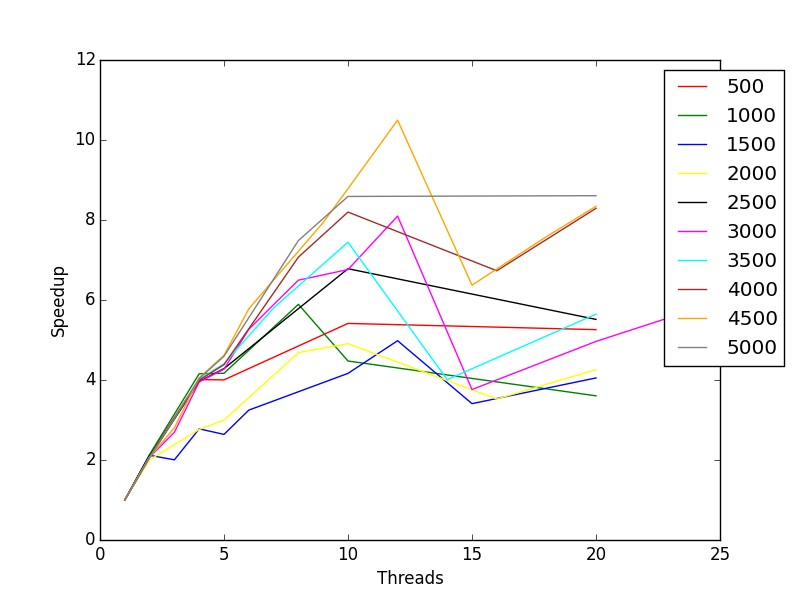
\includegraphics[width=0.68\textwidth] {plots/1}
        \end{center}
      \label{aload0}
      \caption{Strong scaling speedup of our MPI code as number of threads (ranks) increase. Baseline for calculating speedup is MPI with 1 rank}
  \end{subfigure}
  \begin{subfigure}
      \centering
        \begin{center}
      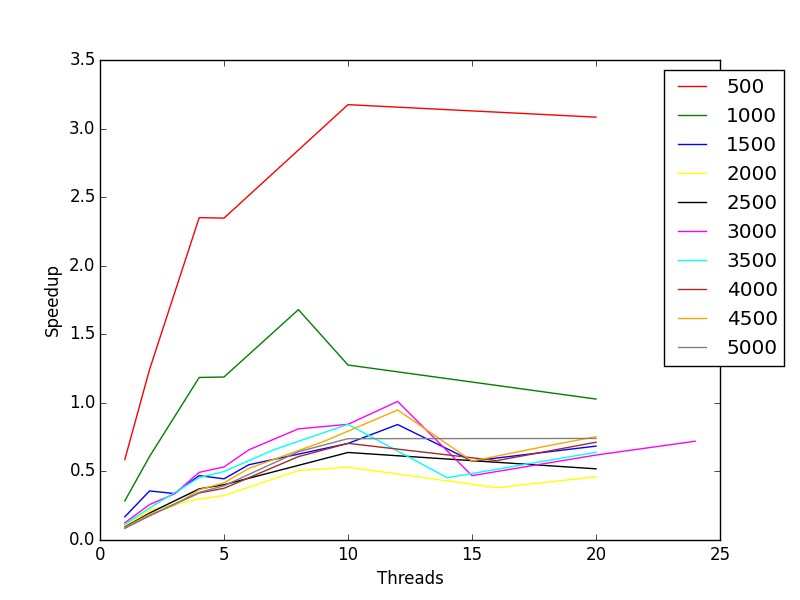
\includegraphics[width=0.68\textwidth] {plots/2}
        \end{center}
      \label{aload1}
      \caption{Strong scaling speedup of our MPI code as number of threads (ranks) increase. Baseline for calculating speedup is OMP with 24 threads.}
  \end{subfigure}

\end{figure}

In Figure 1 we show the results of running our MPI code for various problem sizes and showing how speedup scales as we increase the number of MPI ranks. Larger problems tend to have greater speedup than smaller ones. This makes sense as when we increase problem size less time increase spent in synchronization as compared to actually computation. This means as we increase the number of ranks we should continue to speedup as synchronization does not grow as quickly. The drop seen in speedup when we go beyond 12 ranks is due to now having ranks on 2 chips rather than 1 chip. This increases communication overhead during synchronization which results in a lower overall speedup despite having more cores.

We also compared the performance of our MPI code with that of OMP, where omp was allowed to use all 24 threads (Figure 2) in a strong scaling study. We see that for the two smallest problem sizes our code outperforms OMP as ranks increase beyond 1, but for larger problems our MPI code always performs worse. This is unsurprising as for small problems OMP will have a lot of synchronization overhead for 24 threads while MPI will do better with a smaller problem. However, when the problem is larger MPI, which has a larger synchronization overhead than OMP, MPI performs worse.





\section{Hybrid (MPI and OMP)}

\subsection{Implementation}

MPI and OMP interact seamlessly when put together, making it easy to combine our MPI implementation and the origin OMP implementation. Given a fixed number of MPI ranks, $r$, and $p$ available threads then each MPI rank will have access to $p/r$ threads which can be used in OMP parallel sections of code. This can mean we do not take full advantage of all threads available to us if $p$ is not divisible by $r$. We implemented a hybrid version (by combining our MPI implementation and the OMP parts of the original implementation) in \texttt{path-mpi-omp.c}

\subsection{Performance}

To study the performance of our hybrid code we did strong scaling studies for a large range of n and used baselines of our hybride code with 1 MPI rank (Figure 3), our MPI code with 1 MPI rank (Figure 4), and the given OMP code with 24 OMP threads available (Figure 5).

\begin{figure}[!]
   \begin{subfigure}
      \centering
        \begin{center}
      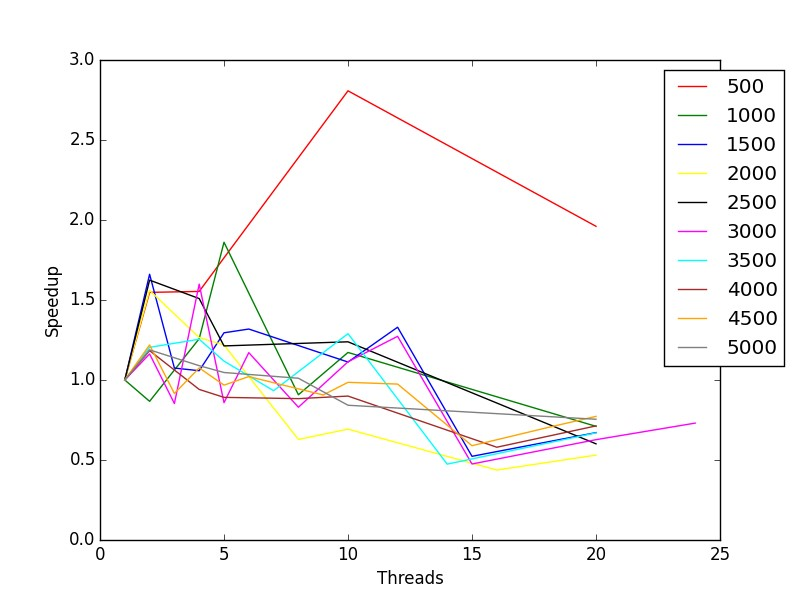
\includegraphics[width=0.63\textwidth] {plots/3}
        \end{center}
      \label{aload0}
      \caption{Strong scaling speedup of our Hybrid code as number of MPI ranks increase (changing the number of available OMP threads to each rank) increase. Baseline for calculating speedup is Hybrid with 1 MPI rank.}
  \end{subfigure}
  \begin{subfigure}
      \centering
        \begin{center}
      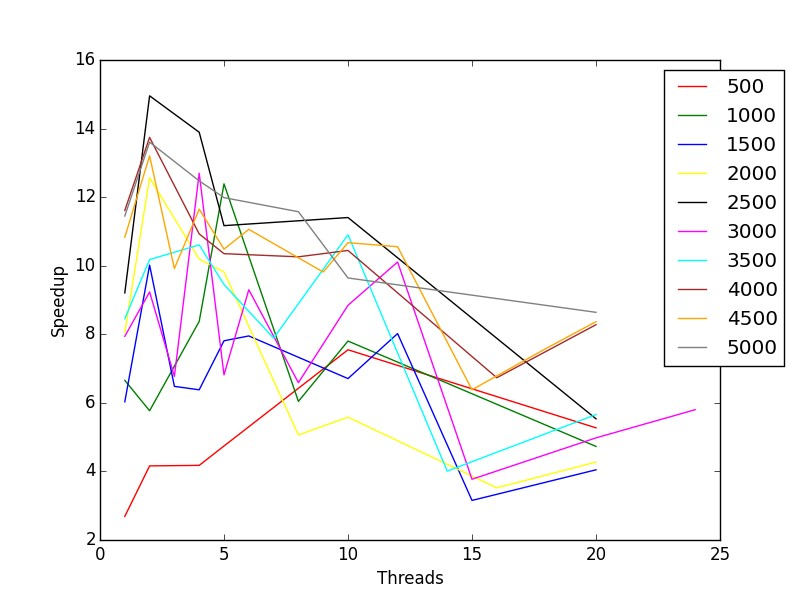
\includegraphics[width=0.63\textwidth] {plots/4}
        \end{center}
      \label{aload1}
      \caption{Strong scaling speedup of our Hybrid code as number of MPI ranks increase (changing the number of available OMP threads to each rank) increase. Baseline for calculating speedup is MPI with 1 MPI rank (thus 1 thread total).}
  \end{subfigure}

\end{figure}

\begin{figure}[!]
\begin{center}
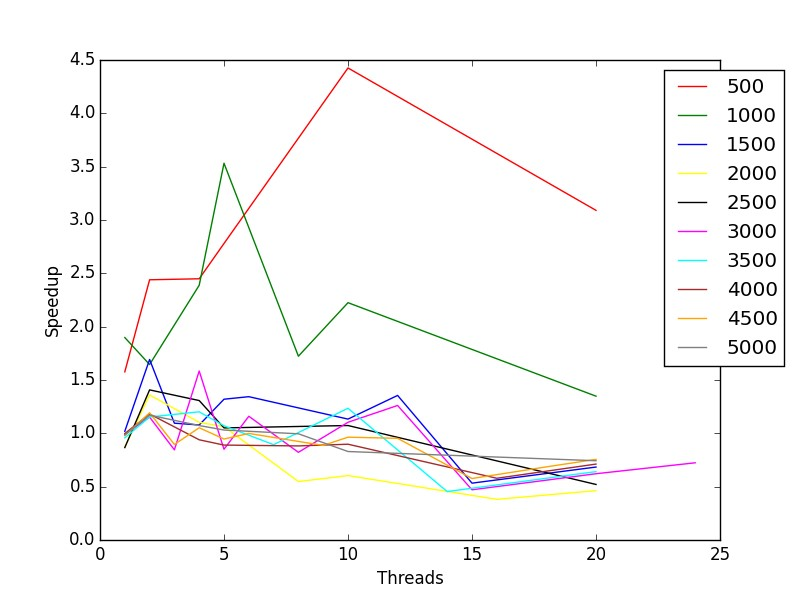
\includegraphics[width=0.65\textwidth]{plots/5}
\caption{Strong scaling speedup of our Hybrid code as number of MPI ranks increase (changing the number of available OMP threads to each rank) increase. Baseline for calculating speedup is OMP code with 24 threads.}
\end{center}
\end{figure}

In Figure 3 we can see that increasing the number of MPI ranks (which in turn decreases the number of OMP threads per rank) has mixed speedup for most n. When the number of MPI ranks is less than 10 we often have speedup larger than 1, but as we go beyond 10 and 12 speedup drops off. This is because of increased MPI overhead across 2 chips and the hybrid codes inability to take advantage of all possible threads when there are more than 12 MPI ranks.

In Figure 4 our hybrid code gets large speedup over the (serial) MPI code (1 rank) for all n. This is because mixing MPI and OMP allows the code to take advantage of more threads than is possible with MPI alone as OMP will take up remaining threads which aren��t allocated to MPI ranks.

In Figure 5 our hybrid code sometimes manages to get speedup of over 1 as compared to  the OMP code. This indicates that mixing MPI and OMP can lead to better thread utilization than using OMP alone.







\section{Floyd$-$Warshall}

\subsection{Implementation}

The algorithm implemented in the original code runs in $O(\log(N)N^3)$ while Floyd$-$Warshall runs in $O(N^3)$. This means in theory that Floyd-Warshall should be significantly faster than the original code. Floyd$-$Warshall is very similar to the original code, except the loop order is $kij$ (or $kji$), As we must calculate the shortest distance using all nodes less than or equal to the current $k$ before calculating for $k+1$. This means the entire set of 3 nested loops cannot be parallelized. Instead only the inner two can. This decreases the amount of parallelism and increases the frequency with which data must be synchronized, while decreasing overall work. We implemented Floyd$-$Warshall (a rather simple set of changes to the original implementation) in both OMP and MPI. Our implementations are in \texttt{fw-omp.c} and \texttt{fw-mpi.c} respectively.

\subsection{Performance}

\begin{figure}[!]
   \begin{subfigure}
      \centering
        \begin{center}
      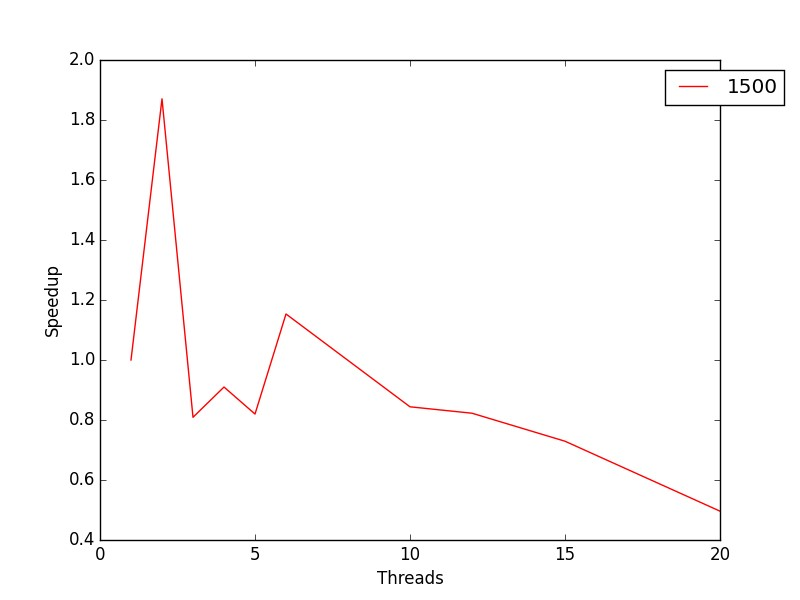
\includegraphics[width=0.68\textwidth] {plots/6}
        \end{center}
      \label{aload0}
      \caption{Strong scaling speedup of our Floyd$-$Warshall MPI code as number of MPI ranks increases. Baseline for calculating speedup is Floyd-Warshall MPI code with 1 rank.}
  \end{subfigure}
  \begin{subfigure}
      \centering
        \begin{center}
      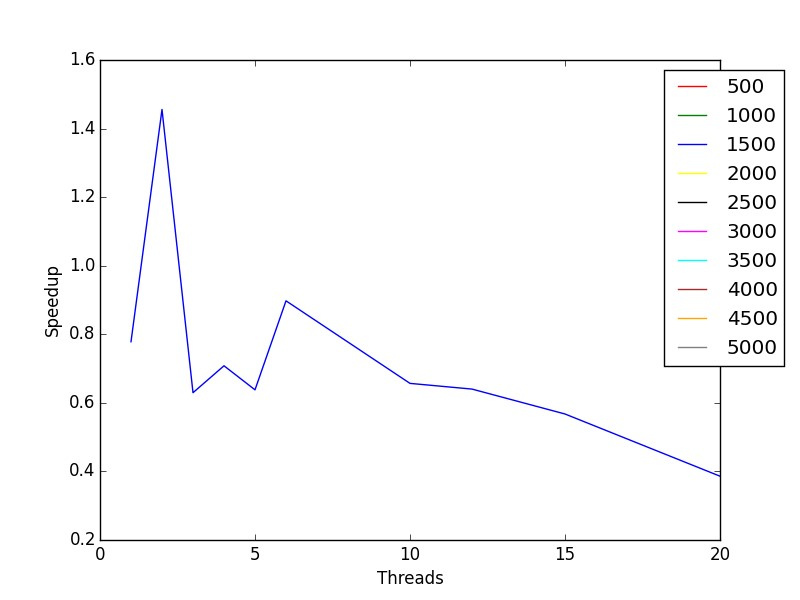
\includegraphics[width=0.68\textwidth] {plots/7}
        \end{center}
      \label{aload1}
      \caption{Strong scaling speedup of our Floyd$-$Warshall MPI code as number of MPI ranks increases. Baseline for calculating speedup is our original MPI code with 1 rank.}
  \end{subfigure}

\end{figure}

We tested our Floyd$-$Warshall code for a single $n$ (1500), as it does not scale well. We calculated strong scaling for this $n$ using a baseline of the Floyd$-$Warshall MPI code with 1 rank (Figure 6) and a baseline of our original MPI code with 1 rank (Figure 7). In Figure 6, the performance of FW MPI increases only until 2 and then starts to drop off. This is for two reasons: the first is the increased overhead once we go beyond 12 ranks (communication across 2 chips is slower) and the larger reason is that communication is expensive in Floyd$-$Warshall. Because we have to synchronize $O(N)$ times rather than $O(\log(N))$ times as we increase the amount of communication that is done (by increasing number of ranks) we see that our code gets slower as we add more parallelism.

In Figure 7 we can see that our speedup is even smaller when compared to our original MPI code, for the exact same reason as before: The extra communication is a major cost and results in a decline in performance as rank increases.







\section{Future Work}

$\bullet$ \quad Run MPI and Hybrid code on the Phis (we have tried extensively, see Piazza at https://piazza.com/class/idnfrkepvo66nw?cid=135)
\\
$\bullet$ \quad Further tune serial parts of algorithm by blocking
\\
$\bullet$ \quad Further parallelize serial parts of algorithm in blocking





\section*{Reference}

(1) D. Bindel, All-Pairs Shortest Paths, Applications of Parallel Computers (CS 5220), Fall 2015.
\\
(2) Floyd$-$Warshall algorithm, https://en.wikipedia.org/wiki/Floyd$-$Warshall\_algorithm, Wikipedia.







\end{document}





